A base matemática para o Método dos Elementos Finitos tem início em 1909 com
Ritz em que um problema contínuo é substituído por um problema discreto
com número finito de graus de liberdade onde as variáveis do problema eram aproximadas
pelo produto entre as constantes a serem determinadas e as funções bases escolhidas de modo 
a garantir a precisão do resultado.
Tal procedimento fica conhecido como \textit{formulação variacional}.
Anos mais tarde, Galerkin utiliza o Método do Resíduo Ponderado na determinação
das constantes da formulação variacional onde as mesmas funções bases foram utilizadas
nas funções peso. Este procedimento fica conhecido como \textit{Formulação de Galerkin}
e é largamente utilizado até hoje.

\medskip
Durante a década de 40, Courant (1943) \cite{courant1943} aplica a formulação variacional em um domínio discretizado
por elementos triangulares. Em 1965, Zienkicwicz e Cheung \cite{zienkiewicz1965} apresentam
que o Método do Resíduo Ponderado possui uma boa aproximação da solução e 
o Método dos Elementos Finitos foi formalizado 
para resolver diversos problemas. A abordagem matemática proposta é frequentemente utilizada nos dias atuais.

\medskip
O Método dos Elementos Finitos se tornou uma ferramenta bastante eficaz na solução de diversos problemas e
foi largamente utilizado em problemas da mecânica dos sólidos. Na mecânica dos fluidos, porém, seu uso só se tornou
possível mais adiante devido às oscilações espúrias que surgiam quando o termo convectivo era superior ao termo
difusivo. Tais oscilações estão presentes não apenas no Método dos Elementos Finitos mas
foram observadas também no Método das Diferenças Finitas por Spalding em 1972 \cite{spalding1972}
onde é apresentado que o efeito \textit{upwind} ajudava na redução dessas oscilações.  

\medskip
Em 1976, Christie et al. \cite{christie1976} modificam as funções peso para funções assimétricas ou quadráticas 
para contornar as oscilações espúrias
em problemas unidimensionais do tipo difusão-convecção. Tais modificações produziam um efeito 
\textit{upwind} na solução. 
Este procedimento ficou conhecido como \textit{Formulação Petrov-Galerkin}. 
No ano seguinte, Heinrich, Huyakorn e Zienkiewicz \cite{heinrich1977} generalizam o esquema para um problema bidimensional.
As matrizes globais, porém, passaram a ser assimétricas diferentemente daquelas apresentadas
no esquema Galerkin.

\medskip
Em 1982, Brooks e Hughes \cite{brooks1982} propõem uma nova formulação que consiste em modificar as 
funções peso de modo que o operador de
difusão atue apenas na direção do escoamento. Este procedimento surge com o intuito de 
eliminar o excesso de difusão perpendicular
ao escoamento que o esquema Petrov-Galerkin apresentava em alguns casos. A formulação 
não requer o uso de funções peso de 
alta ordem e se apresentou eficiente na eliminação da difusão perpendicular. A formulação 
recebeu o nome \textit{Streamline Upwind Petrov-Galerkin} (SUPG).

\medskip
No mesmo ano, Pironneau \cite{pironneau1982} apresenta o Método das Curvas Características
aplicado ao Método dos Elementos Finitos na resolução das equações de convecção-difusão transiente
e Navier-Stokes. Dessa forma o autor foi capaz de derivar esquemas conservativos 
do tipo \textit{upwind} com precisão de primeira e segunda ordem. 
Como as matrizes são simétricas, esse esquema
se apresentou vantajoso na resolução de sistemas lineares em comparação com outros esquemas \textit{upwind}.
A implementação numérica, porém, requer uma integração numérica na montagem dos vetores
do lado direito da equação. Este esquema dá início a diversos trabalhos e 
fica conhecido mais adiante como \textit{Galerkin Característico}.

\medskip
Em 1984, Donea \cite{donea1984} apresenta uma alternativa para a resolução de problemas 
convecção-difusão multidimensionais e transientes.
Tal alternativa é conhecida como esquema \textit{Taylor-Galerkin}.
O esquema consiste em utilizar os termos de alta ordem da expansão de Taylor 
para atuar na redução das oscilações espúrias.
Diferente dos esquemas upwind, no esquema Taylor-Galerkin não há a necessidade 
de usar funções peso modificadas.
O esquema é comparado com as formulações de Galerkin e Petrov-Galerkin 
e apresentou alta precisão e com baixa difusão numérica.
Embora os procedimentos de discretização dos esquemas Taylor-Galerkin e Galerkin Característico
sejam distintos, o sistema de equações é idêntico para a equação de convecção-difusão, onde 
a variável é um escalar como mencionado por Lohner \cite{lohner1984}. 

\medskip
Diversos pesquisadores têm analisado a estabilidade e convergência desses esquemas
e até mesmo a implementação de esquemas mais eficientes tem surgido, como a simulação
numérica apresentada por Anjos et at. em 2006 \cite{anjos2006}, 
em que o esquema \textit{semi-Lagrangeano} é implementado
na modelagem de escoamentos acoplados ao transporte de espécie química numa abordagem
em Elementos Finitos. Este esquema era utilizado largamente na meteorologia e
consiste em calcular a derivada substancial ao longo da trajetória característica.
A discretização no tempo é feita por diferenças regressivas de primeira ordem
enquanto a discretização no espaço é realizada segundo o esquema de Galerkin.
Os resultados mostraram que o esquema semi-Lagrangeano é estável, não apresentando
oscilações espúrias e difusão numérica excessiva mesmo para passos de tempos longos 
e para elevados números de Reynolds e Schmidt. As oscilações espúrias nos esquemas Galerkin, SUPG e semi-Lagrangeano é comparado
por Silva (2011) \cite{silva2011} e é apresentado na \ref{procedimentos oscilacoes espurias}.

\begin{figure}[H]
     \begin{minipage}{.32\linewidth}
      \centering
      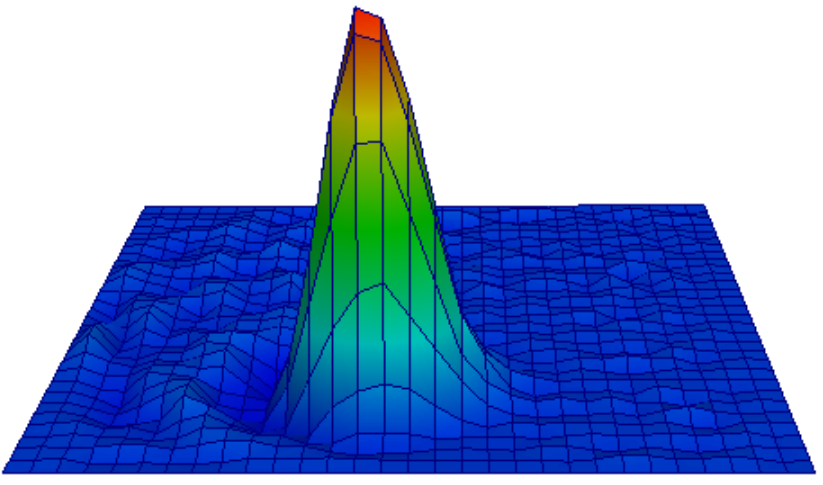
\includegraphics[scale=0.15]{./02_chaps/cap_review/figure/galerkin.png}\\
      (a)
     \end{minipage}%
     \begin{minipage}{.32\linewidth}
      \centering
      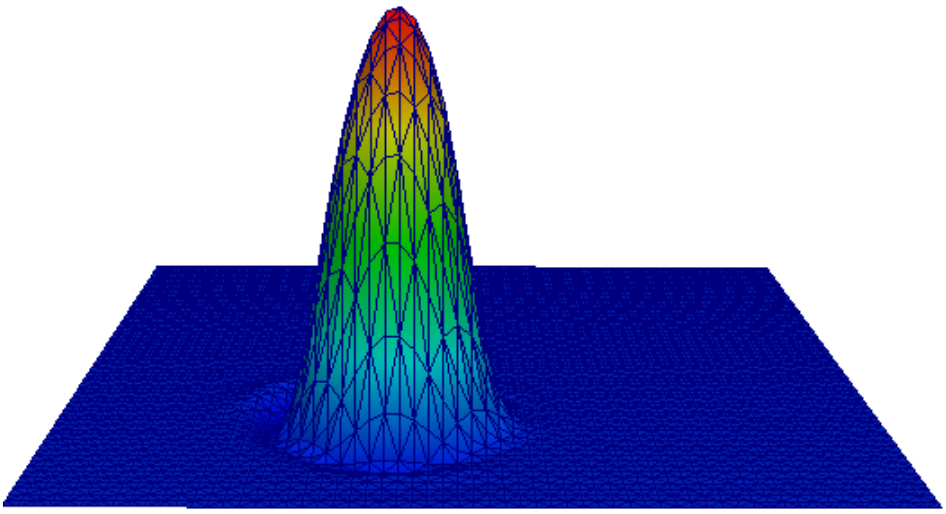
\includegraphics[scale=0.15]{./02_chaps/cap_review/figure/SUPG.png}\\
      (b)
     \end{minipage}%
     \begin{minipage}{.35\linewidth}
      \centering
      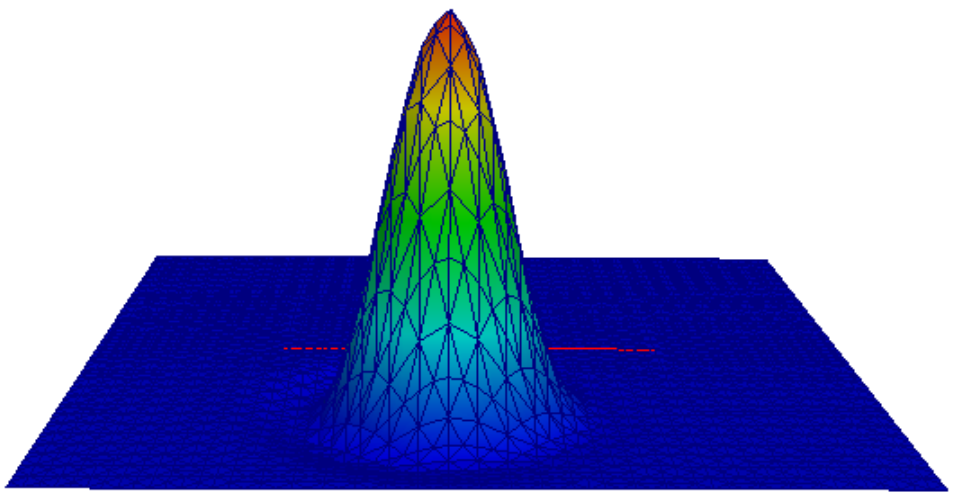
\includegraphics[scale=0.15]{./02_chaps/cap_review/figure/semilagrangian.png}\\
      (c)
     \end{minipage}%
     \medskip
     \caption{Comparativo das oscilações espúrias dos esquemas \cite{silva2011}:
              (a) Galerkin,
              (b) SUPG e 
              (c) semi-Lagrangeano.}
     \label{procedimentos oscilacoes espurias}
\end{figure}



\medskip
A escolha do esquema a ser usado para a redução das oscilações espúrias está relacionado
às suas vantagens e desvantagens quando comparados aos outros esquemas.
Em comparação aos esquemas Petrov-Galerkin e SUPG, os esquemas Taylor-Galerkin,
Galerkin Característico e semi-Lagrangeano possuem a vantagem
de gerar matrizes simétricas facilitando a implementação computacional.
Enquanto isso, embora a eficácia do esquema semi-Lagrangeano seja bem conhecida, o mesmo necessita
de um algoritmo eficiente de busca dos nós vizinhos para realizar a interpolação. Porém nos esquemas Taylor-Galerkin
e Galerkin Característico essa necessidade não existe, assim a implementação computacional torna-se mais simples.
Além disso, o sistema de equações lineares gerados pelo esquema Taylor-Galerkin 
é semelhante àquele gerado pelo esquema Galerkin Característico quando as variáveis são escalares. 
Dessa forma, a escolha entre esses dois esquemas é de cunho pessoal já que produzem
resultados semelhantes embora o processo de discretização seja distinto.

\medskip
Todos os esquemas apresentados possuem resultados bastante satisfatórios
e são bem conhecidos na literatura. Esses esquemas, portanto,
possibilitaram a resolução dos problemas convectivos utilizando a abordagem de Elementos Finitos. 
O esquema Taylor-Galerkin foi escolhido para as simulações apresentadas neste trabalho. 

